\documentclass[11pt]{article}

% Language setting
\usepackage[turkish]{babel}
\usepackage{pythonhighlight}

\usepackage[a4paper,top=2cm,bottom=2cm,left=2cm,right=2cm,marginparwidth=2cm]{geometry}

% Useful packages
\usepackage{amsmath}
\usepackage{graphicx}
\usepackage[colorlinks=true, allcolors=blue]{hyperref}
\usepackage{verbatim}
\usepackage{fancyhdr} % for header and footer
\usepackage{titlesec}
\usepackage{parskip}

\setlength{\parindent}{0pt}

\titleformat{\subsection}[runin]{\bfseries}{\thesubsection}{1em}{}

\pagestyle{fancy} % activate the custom header/footer

% define the header/footer contents
\lhead{\small{23BLM-4014 Yapay Sinir Ağları Ara Sınav Soru ve Cevap Kağıdı}}
\rhead{\small{Dr. Ulya Bayram}}
\lfoot{}
\rfoot{}

% remove header/footer on first page
\fancypagestyle{firstpage}{
  \lhead{}
  \rhead{}
  \lfoot{}
  \rfoot{\thepage}
}
 

\title{Çanakkale Onsekiz Mart Üniversitesi, Mühendislik Fakültesi, Bilgisayar Mühendisliği Akademik Dönem 2022-2023\\
Ders: BLM-4014 Yapay Sinir Ağları/Bahar Dönemi\\ 
ARA SINAV SORU VE CEVAP KAĞIDI\\
Dersi Veren Öğretim Elemanı: Dr. Öğretim Üyesi Ulya Bayram}
\author{%
\begin{minipage}{\textwidth}
\raggedright
Öğrenci Adı Soyadı: Rümeysa Akbaş\\ % Adınızı soyadınızı ve öğrenci numaranızı noktaların yerine yazın
Öğrenci No: 190401003
\end{minipage}%
}

\date{14 Nisan 2023}

\begin{document}
\maketitle

\vspace{-.5in}
\section*{Açıklamalar:}
\begin{itemize}
    \item Vizeyi çözüp, üzerinde aynı sorular, sizin cevaplar ve sonuçlar olan versiyonunu bu formatta PDF olarak, Teams üzerinden açtığım assignment kısmına yüklemeniz gerekiyor. Bu bahsi geçen PDF'i oluşturmak için LaTeX kullandıysanız, tex dosyasının da yer aldığı Github linkini de ödevin en başına (aşağı url olarak) eklerseniz bonus 5 Puan! (Tavsiye: Overleaf)
    \item Çözümlerde ya da çözümlerin kontrolünü yapmada internetten faydalanmak, ChatGPT gibi servisleri kullanmak serbest. Fakat, herkesin çözümü kendi emeğinden oluşmak zorunda. Çözümlerinizi, cevaplarınızı aşağıda belirttiğim tarih ve saate kadar kimseyle paylaşmayınız. 
    \item Kopyayı önlemek için Github repository'lerinizin hiçbirini \textbf{14 Nisan 2023, saat 15:00'a kadar halka açık (public) yapmayınız!} (Assignment son yükleme saati 13:00 ama internet bağlantısı sorunları olabilir diye en fazla ekstra 2 saat daha vaktiniz var. \textbf{Fakat 13:00 - 15:00 arası yüklemelerden -5 puan!}
    \item Ek puan almak için sağlayacağınız tüm Github repository'lerini \textbf{en geç 15 Nisan 2023 15:00'da halka açık (public) yapmış olun linklerden puan alabilmek için!}
    \item \textbf{14 Nisan 2023, saat 15:00'dan sonra gönderilen vizeler değerlendirilmeye alınmayacak, vize notu olarak 0 (sıfır) verilecektir!} Son anda internet bağlantısı gibi sebeplerden sıfır almayı önlemek için assignment kısmından ara ara çözümlerinizi yükleyebilirsiniz yedekleme için. Verilen son tarih/saatte (14 Nisan 2023, saat 15:00) sistemdeki en son yüklü PDF geçerli olacak.
    \item Çözümlerin ve kodların size ait ve özgün olup olmadığını kontrol eden bir algoritma kullanılacaktır. Kopya çektiği belirlenen vizeler otomatikman 0 (sıfır) alacaktır. Bu nedenle çözümlerinizi ve kodlarınızı yukarıda sağladığım gün ve saatlere kadar kimseyle paylaşmayınız.
    \item Bu vizeden alınabilecek en yüksek not 100'dür. Toplam aldığınız puan 100'ü geçerse, aldığınız not 100'e sabitlenecektir.
    \item LaTeX kullanarak PDF oluşturanlar öz geçmişlerine LaTeX bildiklerini de eklemeyi unutmasınlar :)
    \item Bu vizedeki soruların çözümleri ve tex dosyası için istediğiniz kadar sayıda Github repository'si oluşturabilirsiniz. Sadece yukarıda belirttiğim tarihlerde (14 Nisan 2023 saat 15:00 ile 15 Nisan 2023 saat 15:00 arasında) public yapmayı/halka açmayı ve Github profilinizi de öz geçmişinize eklemeyi unutmayın :)
    \item Bilgisayarınıza hiçbir program kurmadan, Overleaf, Google Colab, Kaggle gibi ortamlar üzerinden bu vizeyi tamamlamanız mümkün. İyi çalışmalar!!
\end{itemize}

(Ekstra 5 puan) \url{OdevinTexDosyasınınGithubLinkiniburayakoyun.com}

\newpage
\section{(Toplam 10 Puan) Hopfield Networks:}

\subsection{(2 Puan)} \textbf{ChatGPT’ye size Hopfield Network’ler ile ilgili detaylı bilgi vermesini isteyin. Sorduğunuz soruyu, ChatGPT'nin çıkartığı cevabı aşağı koyun. Bu cevapta anlamadığınız terimleri de ChatGPT’ye sorup, sorduğunuz soruları ve ChatGPT’nin verdiği cevapları da sırayla aşağı koyun.}


\begin{itemize}
    \item Hopfield Networklerle ilgili detaylı bilgi ver.\\
\end{itemize}
Hopfield ağları, biyolojik sinir ağlarından esinlenerek geliştirilmiş bir tür yapay sinir ağıdır. Bu ağlar, öğrenme ve hatırlama işlevlerini gerçekleştirebilen, geri beslemeli bir ağ yapısına sahiptir.

Hopfield ağları, öğrenme sürecindeki örnekleri belleklerinde saklayabilir ve hatırlama işleminde bu örnekleri hatırlayarak sonuç üretebilirler. Bu nedenle, Hopfield ağları özellikle örüntü tanıma ve hatırlama problemlerinde kullanılır.

Hopfield ağları, nöronların birbirleriyle tam bağlantılı olduğu bir ağ yapısına sahiptir. Her nöron, diğer tüm nöronlardan gelen girdileri alır ve çıkışını hesaplar. Nöronların çıkışları, diğer nöronların girdilerine geri beslenir, böylece ağın çıktısı sürekli olarak güncellenir.

Hopfield ağları, öğrenme sürecinde, örneklerin ağırlıklarını hesaplar. Bu ağırlıklar, örneklerin aralarındaki benzerliklere göre belirlenir. Daha sonra, hatırlama işlemi sırasında, ağın girdisi, saklanan örneklerin bir kombinasyonudur ve ağ, bu girdiye uygun bir çıktı üretir.

Hopfield ağları, özellikle küçük boyutlu örneklerle iyi çalışır ve büyük boyutlu örneklerde performansı düşer. Ayrıca, ağın öğrenme sürecindeki hafıza kapasitesi sınırlıdır ve ağ, öğrenilen örneklerin biraz değişik versiyonlarını hatırlayabilir. Bununla birlikte, Hopfield ağları, basit yapısı ve güçlü hatırlama işlevleri nedeniyle halen popüler bir yapay sinir ağı türüdür.


\begin{itemize}
    \item Hopfield Networklerin diğer yapay sinir ağlarından farkı nedir?\\
\end{itemize}
Hopfield ağları, yapay sinir ağları sınıfına ait bir türdür. Yapay sinir ağları, biyolojik sinir ağlarından esinlenerek geliştirilmiş yapay ağlardır ve öğrenme, sınıflandırma, regresyon, örüntü tanıma, veri sıkıştırma, robotik ve diğer uygulamalarda kullanılır.

Hopfield ağları, diğer yapay sinir ağlarından bazı farklılıklara sahiptir. İşlevleri, öğrenme ve hatırlama işlevleri ile sınırlıdır ve diğer yapay sinir ağlarındaki gibi bir çıkış katmanı yoktur. Bunun yerine, tüm nöronlar birbiriyle tam bağlantılıdır ve her nöron, diğer tüm nöronlardan gelen girdileri alır ve çıkışını hesaplar. Bu geri beslemeli bir yapıdır ve her bir nöronun çıkışı diğer nöronların girdilerine geri beslenir.

Hopfield ağları, öğrenme sürecinde, örneklerin ağırlıklarını hesaplar. Bu ağırlıklar, örneklerin aralarındaki benzerliklere göre belirlenir. Daha sonra, hatırlama işlemi sırasında, ağın girdisi, saklanan örneklerin bir kombinasyonudur ve ağ, bu girdiye uygun bir çıktı üretir.

Diğer yapay sinir ağı türleri, öğrenme sürecinde farklı algoritmalar kullanarak ağırlıkları ayarlar. Örneğin, geri yayılım ağı (backpropagation neural network), öğrenme sürecinde hata geri yayılımı algoritması kullanır.

Hopfield ağları, diğer yapay sinir ağı türlerine göre daha az öğrenme kapasitesine sahip olabilir. Ancak, basit yapısı ve güçlü hatırlama işlevleri nedeniyle hala popüler bir yapay sinir ağı türüdür.






\subsection{(8 Puan)} \textbf{ChatGPT’nin açıklamalarından ne anladığınızı buraya kendi kelimelerinizle özetleyin. Örneğin ``Hopfield Network nedir? Ne işe yarar? Neden bilmemiz gerekir bunu? Gerçek hayatta kullanılıyor mu?'' gibi. Anlamadığınız kısımlar varsa ve ChatGPT’nin açıklamaları yeterli gelmezse internet dahil farklı kaynaklardan araştırıp, bilgilerin doğruluğunu sorgulamakta serbestsiniz. Konuyu doğru anlayıp anlamamanız puana etki edecektir. Kullandığınız kaynakları da belirtin!}

Hopfield ağları tek katmandan oluşur. Tüm nöronlar birbirine bağlıdır. Bir nöronun outputu diğer nöronlara input olarak gönderilir böylece hassasiyet ve doğruluk artılmış olur. Hopfield ağları özellikle örüntü tanıma ve hatırlama işlemlerinde kullanılır. Bulanık mantık, veri sıkıştırma, şifreleme işlemlerinde, karakter desen eşleştirmelerinde, biyolojik sistemlerin analizinde, el yazı tanıma sistemlerinde ve diğer birçok alanda da kullanılabilir. Bu avantajların yanı sıra hopfield ağları küçük boyutlu verilerle çalışır, büyük boyutlu verilerde performansı düşer. \\
Kaynakalar: \\
ChatGPT \\
Medium: Hopfield Ağ Modeli - Batıncan Gürbüz \url{https://medium.com/@batincangurbuz/hopfield-a%C4%9F-modeli-hopfield-network-hn-ccf1548ca432}
\section{(Toplam 10 Puan) Boltzman Machine:}

\subsection{(2 Puan)} \textbf{ChatGPT’ye size Boltzman Machine ilgili detaylı bilgi vermesini isteyin. Sorduğunuz soruyu, ChatGPT'nin çıkartığı cevabı aşağı koyun. Bu cevapta anlamadığınız terimleri de ChatGPT’ye sorup, sorduğunuz soruları ve ChatGPT’nin verdiği cevapları da sırayla aşağı koyun.}

\begin{itemize}
    \item Boltzman machine nedir, detaylıca bilgi ver.
\end{itemize}
Boltzmann makinesi, kuantum fiziğindeki Boltzmann dağılımı denklemine dayanan bir yapay sinir ağı türüdür. Bu yapay sinir ağı, girdi verileri ile birbirine bağlı rastgele değişkenlerin ağırlıklarını hesaplayarak, veriler arasındaki olası ilişkileri öğrenmeyi hedefler. Boltzmann makinesi, hem gizli hem de görünen katmanlardan oluşan iki katmanlı bir modeldir.

Boltzmann makinesinin çalışma prensibi, rastgele değişkenlerin durumlarının birbirleriyle etkileşimini modellenmeye dayanır. Bu etkileşim, her değişkenin olası durumlarına bağlı olarak ağırlıklandırılır. Bu ağırlıklar, makineye verilen girdi verilerine dayalı olarak belirlenir ve sonuçta, veriler arasındaki ilişkileri öğrenmek için bir model elde edilir.

Boltzmann makinesi, sınıflandırma, özellik çıkarımı, görüntü işleme ve doğal dil işleme gibi birçok uygulama için kullanılabilir. Örneğin, Boltzmann makineleri, görüntü tanıma ve konuşma tanıma gibi örüntü tanıma problemlerinin çözümünde yaygın olarak kullanılır.

Boltzmann makinesi, unsupervised learning (denetimsiz öğrenme) yöntemleri arasında yer alır ve veriler arasındaki olası ilişkileri keşfetmek için kullanılır. Bu nedenle, Boltzmann makinesi, öğrenme süreci boyunca verilerin etkileşimini modellemek için kullanılır ve daha sonra bu model, yeni girdi verilerini analiz etmek için kullanılabilir.

Boltzmann makinesi, öğrenme süreci boyunca rastgele bir süreç kullanır ve bu süreç, Markov zinciri adı verilen bir süreçtir. Bu süreç, makineye verilen girdi verilerine dayalı olarak ağırlıkların güncellenmesine ve sonuçta modelin oluşturulmasına yol açar.

Boltzmann makinesinin avantajı, özellikle unsupervised learning yöntemleri için önemli olan veriler arasındaki olası ilişkileri öğrenmek için kullanılabilmesidir. Ayrıca, Boltzmann makinesi, verilerin doğal özelliklerini öğrenmek için kullanılabilir ve bu nedenle, özellik çıkarımı gibi birçok uygulama için yararlıdır.
\begin{itemize}
    \item Boltzman dağılımı denklemi nedir?
\end{itemize}
Boltzmann dağılımı, istatistiksel mekanikte kullanılan bir dağılım fonksiyonudur. Boltzmann dağılımı, bir sistemin termodinamik denge halindeki durumunu tanımlamak için kullanılır. Boltzmann makineleri de bu dağılım fonksiyonundan ismini almıştır.
\begin{itemize}
    \item Markov zinciri nedir?
\end{itemize}
Markov zinciri, gelecekteki bir olayın olasılığının, sadece mevcut durumunun bilgisine dayanarak belirlendiği bir matematiksel modeldir. Bu model, belirli bir zaman aralığında meydana gelen olayların sıralamasına dayanarak, olayların olasılıklarını hesaplamak için kullanılır.

Markov zincirleri, zaman içindeki değişimleri modellemek için kullanılır. Her bir durum, bir önceki duruma bağlıdır ve her bir durumun olasılığı, yalnızca önceki durumun bilgisine dayanır. Bu nedenle, Markov zincirleri "geçmişi unutur" ve sadece mevcut duruma dayalı olarak gelecekteki olayların olasılığını hesaplar.

Markov zincirleri, birçok farklı alanda kullanılır. Örneğin, finansal piyasaların analizinde, hava durumu tahmininde, doğal dil işlemede, tıbbi teşhislerde ve mühendislikte kullanılır. Ayrıca, özellikle yapay zeka ve makine öğrenmesi alanlarında, Markov zincirleri, çeşitli uygulamalar için temel bir modelleme aracı olarak da kullanılır.

\subsection{(8 Puan)} \textbf{ChatGPT’nin açıklamalarından ne anladığınızı buraya kendi kelimelerinizle özetleyin. Örneğin ``Boltzman Machine nedir? Ne işe yarar? Neden bilmemiz gerekir bunu? Gerçek hayatta kullanılıyor mu?'' gibi. Anlamadığınız kısımlar varsa ve ChatGPT’nin açıklamaları yeterli gelmezse internet dahil farklı kaynaklardan araştırıp, bilgilerin doğruluğunu sorgulamakta serbestsiniz. Konuyu doğru anlayıp anlamamanız puana etki edecektir. Kullandığınız kaynakları da belirtin!}

Boltman machinelerde hidden layer ve visible layer vardır. Hidden Layer, girdi olarak verilen verileri, visible layer çıktı olarak verilen verileri ifade eder. Hidden layerdaki nöronlar visible layerdaki nöronlara ve hidden layerdaki nöronlara bağlıyken, visible layerdaki nöronlar hidden layerdaki nöronlara bağlıdır. Boltman machineleri denetimsiz öğrenme algoritmaları için kullanılır. Görüntü işleme, yüz tanıma, ses tanıma gibi alanlarda kullanılabilir. Büyük verilerle çalışabilir, bununla beraber diğer sinir ağlarından daha yavaş olması bir dezavantajıdır. Günlük hayatta doğrudan kullanımı sınırlıdır, daha çok uygulamaların arka planında çalışır.\\
Kaynaklar:\\
ChatGPT

\section{(Toplam 10 Puan) Markov Assumption ve Markov Chain:}

\subsection{(2 Puan)} \textbf{ChatGPT’ye size Markov assumption ve Markov Chain ilgili detaylı bilgi vermesini isteyin. Sorduğunuz soruyu, ChatGPT'nin çıkartığı cevabı aşağı koyun. Bu cevapta anlamadığınız terimleri de ChatGPT’ye sorup, sorduğunuz soruları ve ChatGPT’nin verdiği cevapları da sırayla aşağı koyun.}

\begin{itemize}
    \item Markov assumption ve Markov Chain nedir, detaylıca bilgi ver.
\end{itemize}
Markov assumption, bir olayın gelecekteki durumu, sadece şimdiki durumu ile ilgilidir ve geçmiş durumları göz önünde bulundurmaz. Yani bir olayın gelecekteki durumu, şimdiki durumu belirleyen bir değişkene bağlıdır ve geçmiş durumlar etkisizdir.

Markov Chain (Markov Zinciri) ise, bir sistemin durumlarının Markov assumption'a uygun olarak değiştiği, birbirine bağlı bir dizi rassal değişkenlerin matematiksel bir modelidir. Markov zinciri, geçmiş durumlar etkisizdir varsayımına uygun olarak, yalnızca bir önceki durumunun gelecekteki durumunu belirlemekte etkili olduğu bir durum yürüyüşüdür.

Markov zinciri, durumların belli bir zaman dilimi içerisinde belirli bir olasılıkla değiştiği bir süreçtir. Bu süreçte, her bir durum, belirli bir olasılıkla, diğer durumlara geçer. Bu geçiş olasılıkları, bir geçiş matrisi (transition matrix) ile ifade edilir. Geçiş matrisi, her bir iki durum arasındaki geçiş olasılıklarını içerir.

Markov zincirleri, özellikle istatistiksel modellemede ve zaman serisi analizinde kullanılır. Örneğin, hava durumu, hisse senetleri ve doğal dil işleme gibi birçok alanda kullanılır.
\begin{itemize}
    \item Rassal değişken ne demektir?
\end{itemize}
Rassal değişken, belirli bir olasılık dağılımına sahip olan bir değişkendir. Bu değişken, olası bir sonuç kümesine karşılık gelen farklı değerler alabilir. Örneğin, bir zar atıldığında, 1, 2, 3, 4, 5 veya 6 sayılarından biri rassal değişken olarak kabul edilebilir. Rassal değişkenler genellikle belirli bir deney veya olayın sonucunu temsil etmek için kullanılır ve bu deney veya olayın sonucu rastgele bir şekilde belirlenir. Rassal değişkenler, olasılık teorisi, istatistik ve makine öğrenmesi gibi birçok alanda kullanılır.

\subsection{(8 Puan)} \textbf{ChatGPT’nin açıklamalarından ne anladığınızı buraya kendi kelimelerinizle özetleyin. Örneğin ``Markov assumption ve Markov Chain nedir? Ne işe yarar? Neden bilmemiz gerekir bunu? Gerçek hayatta kullanılıyor mu?'' gibi. Anlamadığınız kısımlar varsa ve ChatGPT’nin açıklamaları yeterli gelmezse internet dahil farklı kaynaklardan araştırıp, bilgilerin doğruluğunu sorgulamakta serbestsiniz. Konuyu doğru anlayıp anlamamanız puana etki edecektir. Kullandığınız kaynakları da belirtin!}

Markov Chain ve Markov Assumption, Rus matematikçi Andrey Markov tarafından keşfedilmiştir. Markov assumption, bir olayın gelecekteki durumunu yalnızca mevcut duruma bağlı olarak tahmin etmekle ilgilidir. Markov chain bu prensibi kullanarak belirli bir zaman boyunca, bir dizi durumun olasılık dağılımını modeller.  günlük hayatta markov zincirleri hava durumu tahmini, spor tahmini, hisse senedi artış tahmini, akıllı klavyelerde kelime önerileri gibi birçok yerde kullanılabilir. Markov chain, geçerli durum bilgisini saklayıp, geçmiş bilgileri saklamadığı için bellek gereksinimi azdır. Bunun yanında geçmiş bilgileri saklamadığı için, geçmişe dayalı tahminler yapmakta zorlanır. Büyük veri setleriyle de etkili bir şekilde kullanılabilir ancak veri seti büyüdükçe karmaşıklık artar.\\
Kaynaklar:\\
ChatGPT\\
KhanAcademyTurkce - Markov Zincirlerinin Kökeni \url{https://www.youtube.com/watch?v=uP_N6w-eqlI}

\section{(Toplam 20 Puan) Feed Forward:}
 
\begin{itemize}
    \item Forward propagation için, input olarak şu X matrisini verin (tensöre çevirmeyi unutmayın):\\
    $X = \begin{bmatrix}
        1 & 2 & 3\\
        4 & 5 & 6
        \end{bmatrix}$
    Satırlar veriler (sample'lar), kolonlar öznitelikler (feature'lar).
    \item Bir adet hidden layer olsun ve içinde tanh aktivasyon fonksiyonu olsun
    \item Hidden layer'da 50 nöron olsun
    \item Bir adet output layer olsun, tek nöronu olsun ve içinde sigmoid aktivasyon fonksiyonu olsun
\end{itemize}

Tanh fonksiyonu:\\
$f(x) = \frac{exp(x) - exp(-x)}{exp(x) + exp(-x)}$
\vspace{.2in}

Sigmoid fonksiyonu:\\
$f(x) = \frac{1}{1 + exp(-x)}$

\vspace{.2in}
 \textbf{Pytorch kütüphanesi ile, ama kütüphanenin hazır aktivasyon fonksiyonlarını kullanmadan, formülünü verdiğim iki aktivasyon fonksiyonunun kodunu ikinci haftada yaptığımız gibi kendiniz yazarak bu yapay sinir ağını oluşturun ve aşağıdaki üç soruya cevap verin.}
 
\subsection{(10 Puan)} \textbf{Yukarıdaki yapay sinir ağını çalıştırmadan önce pytorch için Seed değerini 1 olarak set edin, kodu aşağıdaki kod bloğuna ve altına da sonucu yapıştırın:}

% Latex'de kod koyabilirsiniz python formatında. Aşağıdaki örnekleri silip içine kendi kodunuzu koyun
\begin{python}
set_seed(seed=1)
DEVICE = set_device()

# input, hidden layer, output layer boyutlari
input_size = 3
hidden_size = 50
output_size = 1

class MLP(torch.nn.Module):
    def __init__(self):
        super().__init__()
        self.fc1 = torch.nn.Linear(input_size, hidden_size)
        self.fc2 = torch.nn.Linear(hidden_size, output_size)
    
    def forward(self, x):
        # hidden layer
        a1 = tanh_func(self.fc1(x))
        # output layer
        z2 = self.fc2(a1)
        a2 = sigmoid_func(z2)
        return a2
        
model = MLP()
X = torch.tensor([[1, 2, 3], [4, 5, 6]], dtype=torch.float32)
output_tensor = model(X)

print(output_tensor)
\end{python}

Random seed 1 has been set. \\
$\begin{bmatrix}0.4892, 0.5566\end{bmatrix}$

\subsection{(5 Puan)} \textbf{Yukarıdaki yapay sinir ağını çalıştırmadan önce Seed değerini öğrenci numaranız olarak değiştirip, kodu aşağıdaki kod bloğuna ve altına da sonucu yapıştırın:}

\begin{python}
set_seed(seed=190401003)
DEVICE = set_device()

# input, hidden layer, output layer boyutlari
input_size = 3
hidden_size = 50
output_size = 1

class MLP(torch.nn.Module):
    def __init__(self):
        super().__init__()
        self.fc1 = torch.nn.Linear(input_size, hidden_size)
        self.fc2 = torch.nn.Linear(hidden_size, output_size)
    
    def forward(self, x):
        # hidden layer
        a1 = tanh_func(self.fc1(x))
        # output layer
        z2 = self.fc2(a1)
        a2 = sigmoid_func(z2)
        return a2
        
model = MLP()
X = torch.tensor([[1, 2, 3], [4, 5, 6]], dtype=torch.float32)
output_tensor = model(X)

print(output_tensor)
\end{python}

Random seed 190401003 has been set.\\
$\begin{bmatrix}0.7549, 0.7899\end{bmatrix}$

\subsection{(5 Puan)} \textbf{Kodlarınızın ve sonuçlarınızın olduğu jupyter notebook'un Github repository'sindeki linkini aşağıdaki url kısmının içine yapıştırın. İlk sayfada belirttiğim gün ve saate kadar halka açık (public) olmasın:}
% size ait Github olmak zorunda, bu vize için ayrı bir github repository'si açıp notebook'u onun içine koyun. Kendine ait olmayıp da arkadaşının notebook'unun linkini paylaşanlar 0 alacak.

\url{https://github.com/rumeysaakbas/NeuralNetworks/blob/main/ysa_s1.ipynb}

\section{(Toplam 40 Puan) Multilayer Perceptron (MLP):} 
\textbf{Bu bölümdeki sorularda benim vize ile beraber paylaştığım Prensesi İyileştir (Cure The Princess) Veri Seti parçaları kullanılacak. Hikaye şöyle (soruyu çözmek için hikaye kısmını okumak zorunda değilsiniz):} 

``Bir zamanlar, çok uzaklarda bir ülkede, ağır bir hastalığa yakalanmış bir prenses yaşarmış. Ülkenin kralı ve kraliçesi onu iyileştirmek için ellerinden gelen her şeyi yapmışlar, ancak denedikleri hiçbir çare işe yaramamış.

Yerel bir grup köylü, herhangi bir hastalığı iyileştirmek için gücü olduğu söylenen bir dizi sihirli malzemeden bahsederek kral ve kraliçeye yaklaşmış. Ancak, köylüler kral ile kraliçeyi, bu malzemelerin etkilerinin patlayıcı olabileceği ve son zamanlarda yaşanan kuraklıklar nedeniyle bu malzemelerden sadece birkaçının herhangi bir zamanda bulunabileceği konusunda uyarmışlar. Ayrıca, sadece deneyimli bir simyacı bu özelliklere sahip patlayıcı ve az bulunan malzemelerin belirli bir kombinasyonunun prensesi iyileştireceğini belirleyebilecekmiş.

Kral ve kraliçe kızlarını kurtarmak için umutsuzlar, bu yüzden ülkedeki en iyi simyacıyı bulmak için yola çıkmışlar. Dağları tepeleri aşmışlar ve nihayet "Yapay Sinir Ağları Uzmanı" olarak bilinen yeni bir sihirli sanatın ustası olarak ün yapmış bir simyacı bulmuşlar.

Simyacı önce köylülerin iddialarını ve her bir malzemenin alınan miktarlarını, ayrıca iyileşmeye yol açıp açmadığını incelemiş. Simyacı biliyormuş ki bu prensesi iyileştirmek için tek bir şansı varmış ve bunu doğru yapmak zorundaymış. (Original source: \url{https://www.kaggle.com/datasets/unmoved/cure-the-princess})

(Buradan itibaren ChatGPT ve Dr. Ulya Bayram'a ait hikayenin devamı)

Simyacı, büyülü bileşenlerin farklı kombinasyonlarını analiz etmek ve denemek için günler harcamış. Sonunda birkaç denemenin ardından prensesi iyileştirecek çeşitli karışım kombinasyonları bulmuş ve bunları bir veri setinde toplamış. Daha sonra bu veri setini eğitim, validasyon ve test setleri olarak üç parçaya ayırmış ve bunun üzerinde bir yapay sinir ağı eğiterek kendi yöntemi ile prensesi iyileştirme ihtimalini hesaplamış ve ikna olunca kral ve kraliçeye haber vermiş. Heyecanlı ve umutlu olan kral ve kraliçe, simyacının prensese hazırladığı ilacı vermesine izin vermiş ve ilaç işe yaramış ve prenses hastalığından kurtulmuş.

Kral ve kraliçe, kızlarının hayatını kurtardığı için simyacıya krallıkta kalması ve çalışmalarına devam etmesi için büyük bir araştırma bütçesi ve çok sayıda GPU'su olan bir server vermiş. İyileşen prenses de kendisini iyileştiren yöntemleri öğrenmeye merak salıp, krallıktaki üniversitenin bilgisayar mühendisliği bölümüne girmiş ve mezun olur olmaz da simyacının yanında, onun araştırma grubunda çalışmaya başlamış. Uzun yıllar birlikte krallıktaki insanlara, hayvanlara ve doğaya faydalı olacak yazılımlar geliştirmişler, ve simyacı emekli olduğunda prenses hem araştırma grubunun hem de krallığın lideri olarak hayatına devam etmiş.

Prenses, kendisini iyileştiren veri setini de, gelecekte onların izinden gidecek bilgisayar mühendisi prensler ve prensesler başkalarına faydalı olabilecek yapay sinir ağları oluşturmayı öğrensinler diye halka açmış ve sınavlarda kullanılmasını salık vermiş.''

\textbf{İki hidden layer'lı bir Multilayer Perceptron (MLP) oluşturun beşinci ve altıncı haftalarda yaptığımız gibi. Hazır aktivasyon fonksiyonlarını kullanmak serbest. İlk hidden layer'da 100, ikinci hidden layer'da 50 nöron olsun. Hidden layer'larda ReLU, output layer'da sigmoid aktivasyonu olsun.}

\textbf{Output layer'da kaç nöron olacağını veri setinden bakıp bulacaksınız. Elbette bu veriye uygun Cross Entropy loss yöntemini uygulayacaksınız. Optimizasyon için Stochastic Gradient Descent yeterli. Epoch sayınızı ve learning rate'i validasyon seti üzerinde denemeler yaparak (loss'lara overfit var mı diye bakarak) kendiniz belirleyeceksiniz. Batch size'ı 16 seçebilirsiniz.}

\subsection{(10 Puan)} \textbf{Bu MLP'nin pytorch ile yazılmış class'ının kodunu aşağı kod bloğuna yapıştırın:}

\begin{python}
class MLP(nn.Module):
    def __init__(self, input_size, h1_size, h2_size, output_size):
        super(MLP, self).__init__()
        self.fc1 = nn.Linear(input_size, h1_size)
        self.fc2 = nn.Linear(h1_size, h2_size)
        self.fc3 = nn.Linear(h2_size, output_size)
        self.relu = nn.ReLU()
        self.sigmoid = nn.Sigmoid()

    def forward(self, input_layer):
        hidden_layer1 = self.relu(self.fc1(input_layer))
        hidden_layer2 = self.relu(self.fc2(hidden_layer1))
        output_layer = self.sigmoid(self.fc3(hidden_layer2))
        return output_layer
\end{python}

\subsection{(10 Puan)} \textbf{SEED=öğrenci numaranız set ettikten sonra altıncı haftada yazdığımız gibi training batch'lerinden eğitim loss'ları, validation batch'lerinden validasyon loss değerlerini hesaplayan kodu aşağıdaki kod bloğuna yapıştırın ve çıkan figürü de alta ekleyin.}

\begin{python}
  for epoch in range(num_epochs):

    # training loop
    train_loss = 0.0
    train_count = 0.0
    for X_train, y_train in trainloader:
        # zero the parameter gradients
        optimizer.zero_grad()

        outputs = model(X_train)
        loss = criterion(outputs, y_train.unsqueeze(1))
        loss += 0.5 * 0.001 * sum([torch.sum(param ** 2) for param in model.parameters()])
        loss.backward()
        optimizer.step()
        train_count += 1.0
        train_loss += loss.item()

    val_loss = 0.0
    with torch.no_grad():
        model.eval()
        for inputs, labels in valloader:
            outputs = model(inputs)
            loss = criterion(outputs, labels)
            #validation_count += 1.0
            val_loss += loss.item()
    model.train()

    # calculate metrics
    train_loss /= train_count
    val_loss /= len(valloader)
    #val_acc = 100 * val_correct / val_total

    print("Epoch", epoch, "Training loss", train_loss,"Validation Loss :",val_loss)
\end{python}

% Figure aşağıda comment içindeki kısımdaki gibi eklenir.
\begin{comment}
\begin{figure}[ht!]
    \centering
    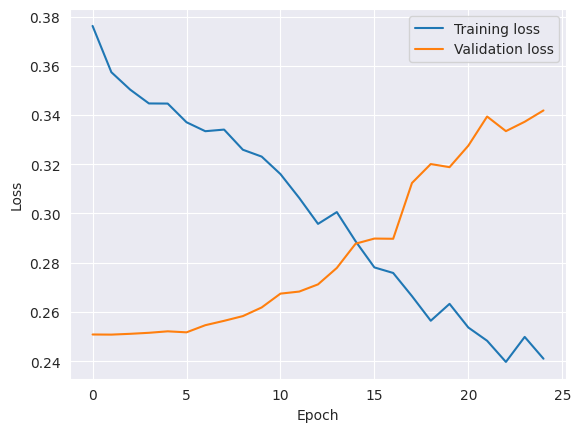
\includegraphics[width=0.75\textwidth]{training_validation_loss.png}
    \caption{Epoch 0 Training loss 0.3762228526175022 Validation Loss : 0.2508285686373711
Epoch 1 Training loss 0.3574111945927143 Validation Loss : 0.25077910274267196
Epoch 2 Training loss 0.35034216940402985 Validation Loss : 0.25110129863023756
Epoch 3 Training loss 0.34471756890416144 Validation Loss : 0.2515166848897934
Epoch 4 Training loss 0.3446684777736664 Validation Loss : 0.25211646109819413
Epoch 5 Training loss 0.33707720041275024 Validation Loss : 0.2517042875289917
...
Epoch 22 Training loss 0.2396813239902258 Validation Loss : 0.3334674537181854
Epoch 23 Training loss 0.24984643198549747 Validation Loss : 0.3372780680656433
Epoch 24 Training loss 0.24098959937691689 Validation Loss : 0.3418796956539154}
    \label{fig:my_pic}
\end{figure}
\end{comment}

\subsection{(10 Puan)} \textbf{SEED=öğrenci numaranız set ettikten sonra altıncı haftada ödev olarak verdiğim gibi earlystopping'deki en iyi modeli kullanarak, Prensesi İyileştir test setinden accuracy, F1, precision ve recall değerlerini hesaplayan kodu yazın ve sonucu da aşağı yapıştırın. \%80'den fazla başarı bekliyorum test setinden. Daha düşükse başarı oranınız, nerede hata yaptığınızı bulmaya çalışın. \%90'dan fazla başarı almak mümkün (ben denedim).}

\begin{python}
from sklearn.metrics import classification_report, confusion_matrix

y_pred = model(X_test)
y_pred = torch.argmax(y_pred, dim=1)

cm = confusion_matrix(y_test, y_pred)
cr = classification_report(y_test, y_pred)

print("Confusion matrix:")
print(cm)
print("\nClassification report:")
print(cr)
\end{python}

Sonuçlar buraya

\begin{figure}
    \centering
    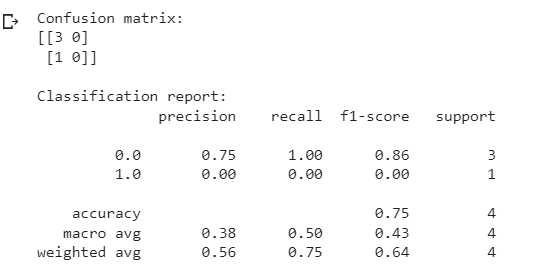
\includegraphics{test.png}
    \caption{Caption}
    \label{fig:my_label}
\end{figure}

\subsection{(5 Puan)} \textbf{Tüm kodların CPU'da çalışması ne kadar sürüyor hesaplayın. Sonra to device yöntemini kullanarak modeli ve verileri GPU'ya atıp kodu bir de böyle çalıştırın ve ne kadar sürdüğünü hesaplayın. Süreleri aşağıdaki tabloya koyun. GPU için Google Colab ya da Kaggle'ı kullanabilirsiniz, iki ortam da her hafta saatlerce GPU hakkı veriyor.}

\begin{table}[ht!]
    \centering
    \caption{Buraya bir açıklama yazın}
    \begin{tabular}{c|c}
        Ortam & Süre (saniye) \\\hline
        CPU & 7.064 \\
        GPU & 3.467\\
    \end{tabular}
    \label{tab:my_table}
\end{table}

\subsection{(3 Puan)} \textbf{Modelin eğitim setine overfit etmesi için elinizden geldiği kadar kodu gereken şekilde değiştirin, validasyon loss'unun açıkça yükselmeye başladığı, training ve validation loss'ları içeren figürü aşağı koyun ve overfit için yaptığınız değişiklikleri aşağı yazın. Overfit, tam bir çanak gibi olmalı ve yükselmeli. Ona göre parametrelerle oynayın.}

Epoch sayısını 25'ten 70'e çıkardım. Learning Rate'i 0.001'den 0.1 e çıkardım ve 0.7 olan dropout değerini 0.2 yaptım.

% Figür aşağı
\begin{comment}
\begin{figure}[ht!]
    \centering
    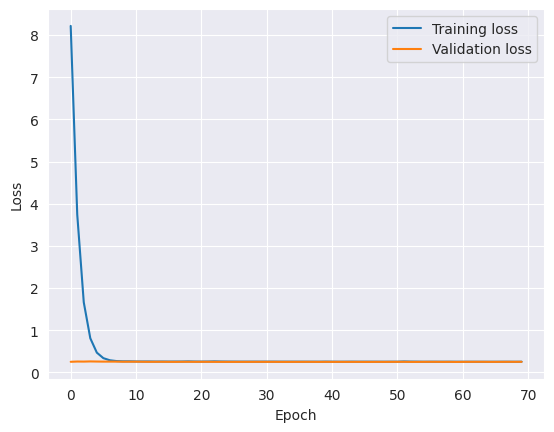
\includegraphics[width=0.75\textwidth]{overfit.png}
    \caption{Buraya açıklama yazın}
    \label{fig:my_pic}
\end{figure}
\end{comment}

\subsection{(2 Puan)} \textbf{Beşinci soruya ait tüm kodların ve cevapların olduğu jupyter notebook'un Github linkini aşağıdaki url'e koyun.}

\url{https://github.com/rumeysaakbas/NeuralNetworks/blob/main/ysa_s2.ipynb}

\section{(Toplam 10 Puan)} \textbf{Bir önceki sorudaki Prensesi İyileştir problemindeki yapay sinir ağınıza seçtiğiniz herhangi iki farklı regülarizasyon yöntemi ekleyin ve aşağıdaki soruları cevaplayın.} 

\subsection{(2 puan)} \textbf{Kodlarda regülarizasyon eklediğiniz kısımları aşağı koyun:} 

\begin{python}
# dropout eklendi
class MLP(nn.Module):
    def __init__(self, input_size, h1_size, h2_size, output_size):
        super(MLP, self).__init__()
        self.fc1 = nn.Linear(input_size, h1_size)
        self.bn1 = nn.BatchNorm1d(h1_size)
        self.fc2 = nn.Linear(h1_size, h2_size)
        self.bn2 = nn.BatchNorm1d(h2_size)
        self.fc3 = nn.Linear(h2_size, output_size)
        self.relu = nn.ReLU()
        self.sigmoid = nn.Sigmoid()
        self.dropout = nn.Dropout(p=0.2)
        
    def forward(self, input_layer):
        hidden_layer1 = self.dropout(self.relu(self.bn1(self.fc1(input_layer))))
        hidden_layer2 = self.dropout(self.relu(self.bn2(self.fc2(hidden_layer1))))
        output_layer = self.sigmoid(self.fc3(hidden_layer2))
        return output_layer
\end{python}
\begin{python}
#L2 regularizasyon eklendi
for epoch in range(num_epochs):
    # training loop
    train_loss = 0.0
    train_count = 0.0
    for X_train, y_train in trainloader:
        # zero the parameter gradients
        optimizer.zero_grad()

        outputs = model(X_train.to(device))
        loss = criterion(outputs, y_train.to(device).unsqueeze(1))
        loss += 0.5 * 0.001 * sum([torch.sum(param ** 2) for param in model.parameters()])
        loss.backward()
        optimizer.step()
        train_count += 1.0
        train_loss += loss.item()
\end{python}

\subsection{(2 puan)} \textbf{Test setinden yeni accuracy, F1, precision ve recall değerlerini hesaplayıp aşağı koyun:}

Sonuçlar buraya.

\subsection{(5 puan)} \textbf{Regülarizasyon yöntemi seçimlerinizin sebeplerini ve sonuçlara etkisini yorumlayın:}

Yorumlar buraya.

\subsection{(1 puan)} \textbf{Sonucun github linkini  aşağıya koyun:}

\url{www.benimgithublinkim2.com}

\end{document}